% Written by Louise Fussien
% This file CAN NOT be compiled on its own
% It is included by ../Book_of_Specifications.tex

\subsection{Design}

\subsubsection{Notre logo}

\textbf{Symbolisme de la couleur jaune}
\vspace*{0.2cm}

Le jaune, au cœur de notre identité visuelle, est choisi avec soin pour ses implications psychologiques profondes et ses associations scientifiquement étayées :
\\

Énergie et dynamisme : Le jaune est universellement reconnu pour son pouvoir d'éveiller l'énergie, la vitalité et le dynamisme. Psychologiquement, cette couleur stimule les sens et incite à l'action. Pour une entreprise de jeux vidéo comme la nôtre, ces qualités sont cruciales pour susciter l'enthousiasme et l'engagement des joueurs, en harmonie avec leurs attentes d'expériences immersives et passionnantes.
\\

Optimisme et positivité : En plus de son énergie palpable, le jaune est une couleur intrinsèquement positive, évoquant la joie, l'optimisme et une attitude lumineuse envers l'avenir. Des études montrent que cette couleur stimule la libération de sérotonine dans le cerveau, neurotransmetteur associé à la régulation de l'humeur et au bien-être. Ainsi, notre choix du jaune reflète non seulement notre dynamisme mais aussi notre désir de créer des expériences de jeu qui inspirent et réconfortent nos joueurs.
\\

\textbf{Deux tons de jaune}
\vspace*{0.2cm}

Contraste et dimension : La dualité de deux nuances de jaune dans notre logo n'est pas uniquement esthétique mais aussi stratégique sur le plan psychologique. Ce contraste subtil mais significatif crée une profondeur visuelle qui attire l'œil et prolonge l'intérêt. La recherche en psychologie de la couleur suggère que l'utilisation de multiples nuances dans une même palette stimule la cognition visuelle, augmentant ainsi la mémorabilité et l'impact du logo.
\\

Accentuation : Le jeu de nuances dans notre logo n'est pas seulement pour l'esthétique, mais aussi pour guider l'attention et renforcer la reconnaissance. Le contraste entre les tons de jaune accentue des éléments clés comme le nom de l'entreprise et les motifs iconographiques, améliorant ainsi la lisibilité et la perception du logo dans divers contextes visuels.
\\

\textbf{Pourquoi un éclair ?}
\vspace*{0.2cm}

Puissance et rapidité : L'éclair, symbole central de notre logo, transcende les frontières culturelles en évoquant la puissance, la rapidité et l'énergie dynamique.
D'un point de vue psychologique, cette forme évoque la perception humaine de la vitesse et de l'action immédiate, des qualités essentielles dans les jeux vidéo où la réactivité est cruciale.
Des études montrent que les formes pointues et dynamiques comme celle de l'éclair activent les zones du cerveau associées à l'attention et à la réaction rapide, renforçant ainsi l'attrait visuel et l'engagement émotionnel envers notre marque.
\\

Technologie et innovation : En plus de sa symbolique dynamique, l'éclair représente également l'innovation technologique et la modernité.
Dans l'univers des jeux vidéo, où la technologie est au cœur de l'expérience, cette icône suggère notre engagement envers l'avant-garde et notre capacité à repousser les limites créatives et techniques pour offrir des expériences de jeu innovantes et captivantes.
\\

Impact visuel : Visuellement frappant, l'éclair captive instantanément l'attention et crée une impression durable.
Cette forme distinctive, par sa nature audacieuse et évocatrice, se distingue dans le paysage visuel saturé d'aujourd'hui, renforçant ainsi la visibilité et la reconnaissance de notre marque.
\\

\textbf{Pourquoi souligné ?}
\vspace*{0.2cm}

Accentuation : Le soulignement stratégiquement placé sous le nom "Stonks" dans notre logo n'est pas seulement décoratif mais fonctionne comme un guide visuel pour l'identification et la mémorisation.
Selon des principes de design psychologique, un élément de soulignement attire naturellement l'œil, aidant à focaliser l'attention sur le nom de l'entreprise et à renforcer sa présence visuelle dans l'esprit des consommateurs.
Par ailleurs, "Stonks" est une expression internet humoristique qui déforme intentionnellement le mot "stocks" (actions en anglais) pour faire référence de manière ironique aux investissements et aux bénéfices financiers.
En français, on pourrait traduire cela par "actions" ou par une expression équivalente comme "les actions qui montent en flèche".
Le jaune accentué à l'illusion de pouvoir ne peut que plaire au public.
\\

Stabilité et structure : Structuralement, le soulignement ajoute une stabilité visuelle au design global du logo, évoquant une fondation solide et une entreprise fiable.
Cette ligne horizontale, en contraste avec les éléments plus dynamiques comme l'éclair, crée un équilibre esthétique qui contribue à une composition harmonieuse et esthétiquement agréable.
\\

Esthétique et équilibre : En harmonisant les éléments diagonaux et courbes de l'éclair avec le soulignement horizontal, notre logo atteint un équilibre visuel qui est à la fois esthétiquement attrayant et fonctionnel.
Ce contraste de formes et de lignes non seulement renforce la composition visuelle mais renforce également l'impact émotionnel et mémoriel de notre marque.

\begin{figure}[H]
      \centering
      
\includegraphics[width=0.3\textwidth]{assets/logo_stonks.png}
      \caption{Le logo de l'entreprise}
      \label{fig:website1}
\end{figure}

\subsubsection{Inspirations Design}

L'esthétique du jeu \textit{Lands of Azerith} est profondément influencée par des classiques du jeu vidéo et des titres emblématiques du pixel art tels que \textit{Stardew Valley} et \textit{Undertale}.
Ces jeux ont non seulement évoqué la nostalgie des genres passés, mais ont aussi démontré la capacité du pixel art à offrir une esthétique artistique distinctive tout en restant léger sur les ressources.
Nous avons également puisé notre inspiration dans d'autres œuvres de pixel art, ce qui nous a permis d'explorer divers styles et techniques pour notre propre projet.
\\

En plus d'évoquer la nostalgie des jeux classiques, le pixel art nous offre une exigibilité artistique tout en étant relativement léger en termes de ressources.
Inspiré par des jeux emblématiques tels que \textit{Stardew Valley}, \textit{Undertale}, ainsi que par d'autres jeux rétro, le choix du style graphique pixel art en 2D pour
\textit{Lands of Azerith} provient du choix réfléchi de l'esthétique du jeu et son potentiel à immerger les joueurs dans un monde magique et riche en aventures.
En effet, ce choix s'est révélé être une décision artistique judicieuse.
Ce style graphique simple et détaillé à la fois confère au jeu un charme unique tout en permettant une représentation qualitative des environnements et des personnages.
De plus, l'atmosphère visuelle du jeu est soigneusement choisie en fonction des différentes zones du jeu pour une meilleure immersion des joueurs dans l'univers apporté par \textit{Lands of Azerith}.

\begin{figure}[H]
      \centering
      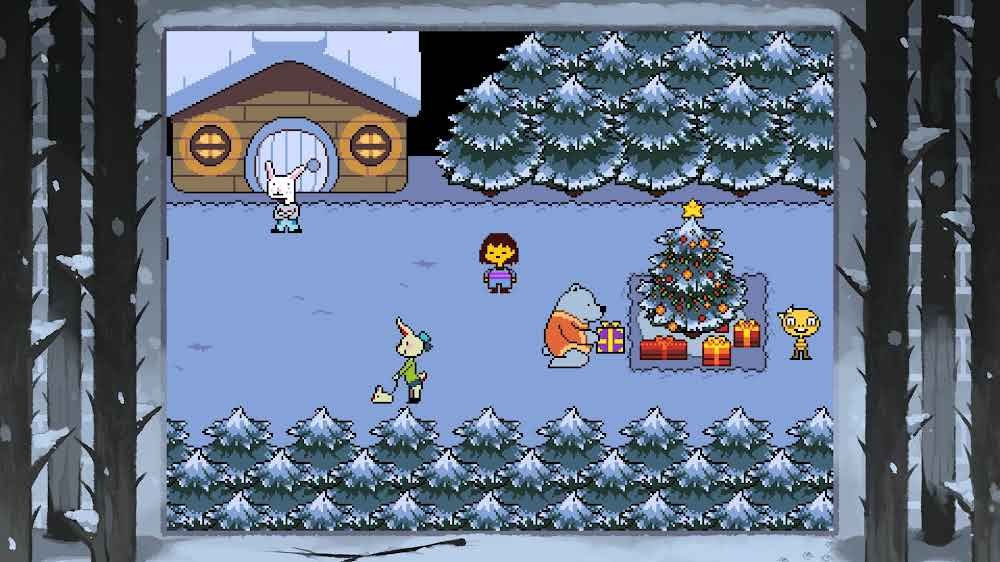
\includegraphics[width=0.8\textwidth]{assets/undertale.png}
      \caption{Exemple du design du jeu Undertale}
      \label{fig:undertale}
\end{figure}

\begin{figure}[H]
      \centering
      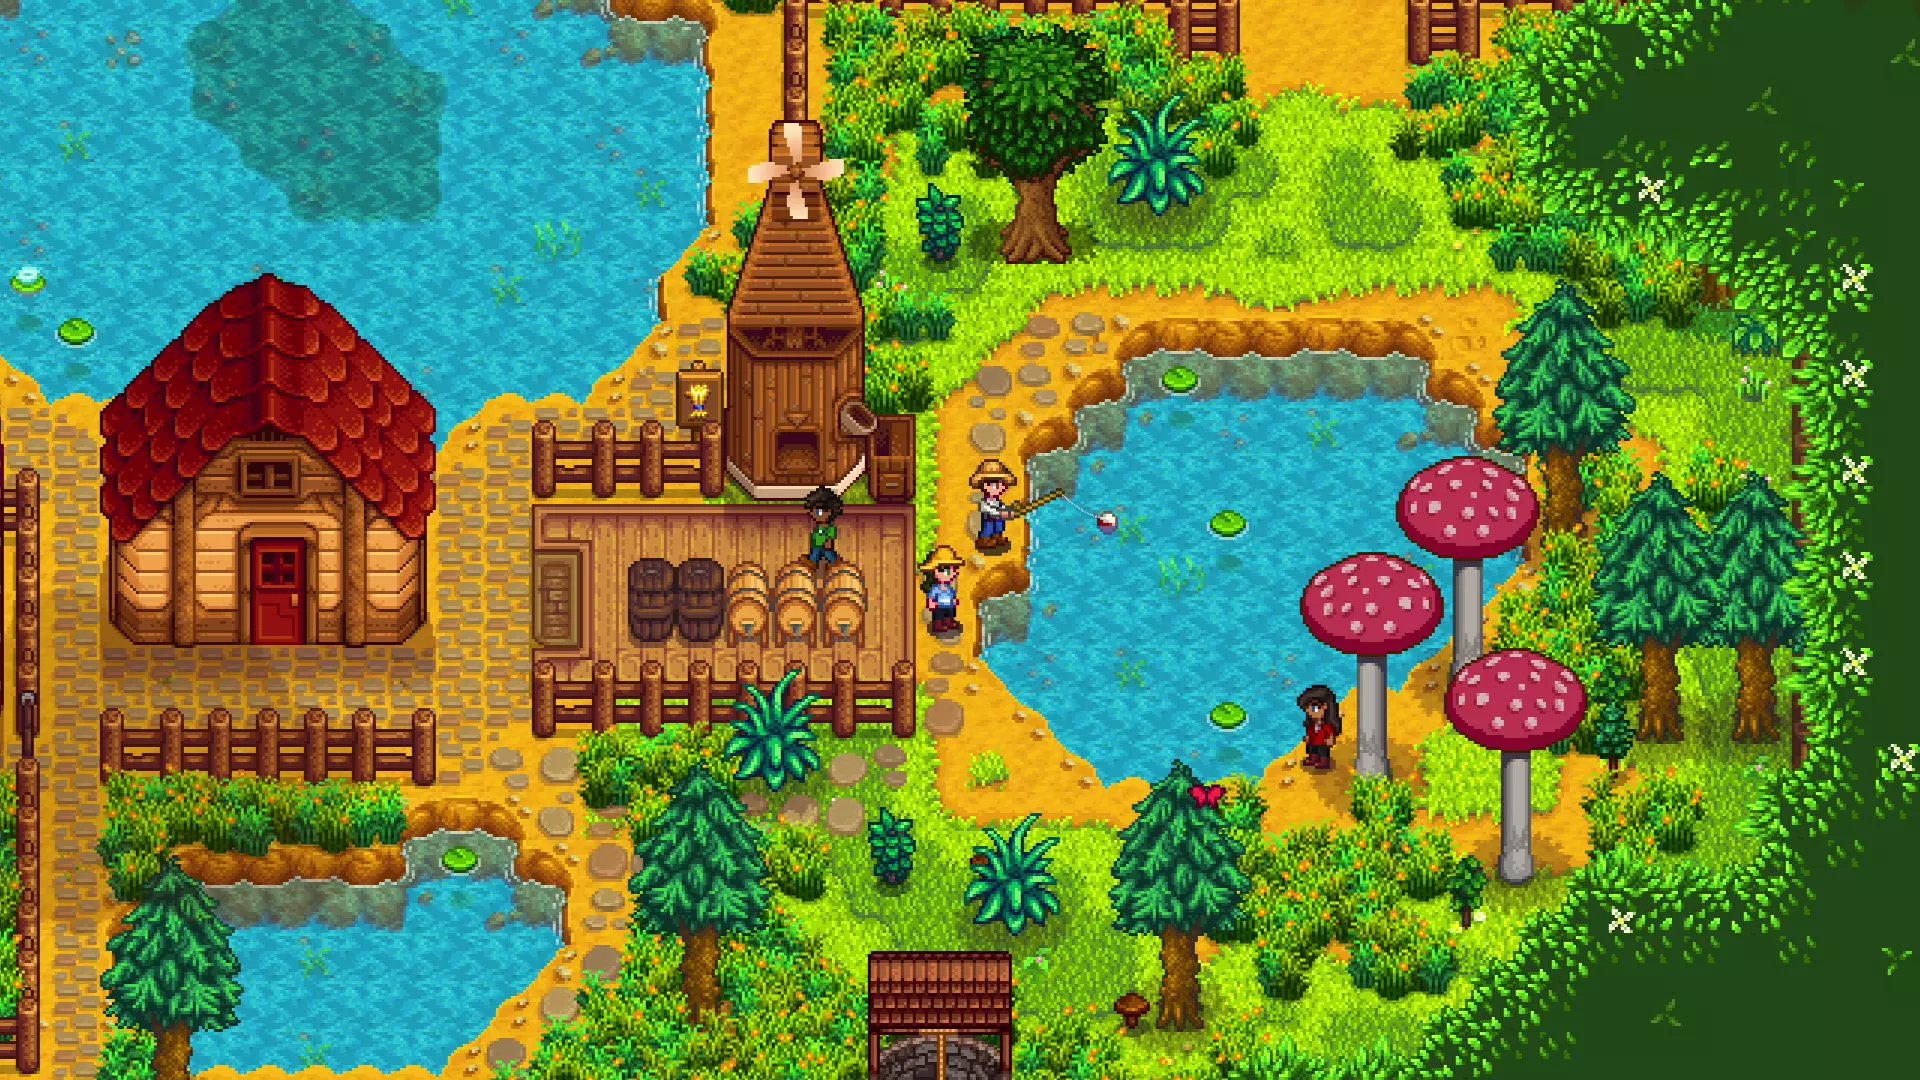
\includegraphics[width=0.8\textwidth]{assets/stardueley.png}
      \caption{Exemple de design du jeu Stardew Valley}
      \label{fig:stardueley}
\end{figure}

\subsubsection{Création et implémentation design}

Le choix du pixel art en 2D pour \textit{Lands of Azerith} découle d'une décision délibérée visant à immerger les joueurs dans un monde magique et riche en aventures.
Ce style graphique combine simplicité et détails minutieux, offrant un charme unique tout en permettant une représentation visuelle de haute qualité des environnements et des personnages du jeu.
Chaque zone du jeu est soigneusement conçue pour refléter une atmosphère distincte, renforçant ainsi l'immersion des joueurs dans un univers captivant.

\textbf{Création des Textures}
\vspace*{0.2cm}

La création des textures pour \textit{Lands of Azerith} a été un processus méticuleux, réalisé avec des outils comme GIMP pour assurer une flexibilité créative maximale.
À partir de concepts initiaux inspirés d'images et de textures d'autres jeux, notre équipe a développé des textures variées pour les environnements, les personnages et les objets du jeu.
Chaque texture est peaufinée avec attention pour enrichir l'expérience visuelle du joueur et garantir une cohérence esthétique à travers le monde de jeu :
\\

\begin{itemize}

      \item \textbf{Conceptualisation et Modélisation :} Exploration d'idées et de concepts pour chaque élément du jeu.
            \\

      \item \textbf{Réalisation des Textures :} Création détaillée des textures en plusieurs itérations pour atteindre le rendu final souhaité.
            \\

      \item \textbf{Intégration et Test :} Validation des textures dans le jeu pour assurer leur intégration harmonieuse et leur impact visuel optimal.
            \\

\end{itemize}

\begin{figure}[H]
      \centering
      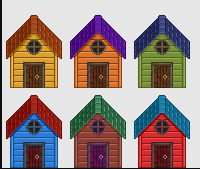
\includegraphics[width=0.35\textwidth]{assets/maison.png}
      \caption{Maisons crées pour le jeu}
      \label{fig:maison}
\end{figure}

\textbf{Intégration des Éléments Graphiques dans le Jeu}
\\

L'intégration des textures et des éléments graphiques joue un rôle crucial dans la création d'une expérience immersive pour les joueurs.
Chaque texture est soigneusement ajustée et testée pour s'assurer qu'elle correspond aux spécifications techniques du jeu et contribue à l'atmosphère globale de \textit{Lands of Azerith}.
Cette étape inclut l'incorporation des textures dans les décors, les personnages et les objets du jeu, garantissant ainsi une cohérence visuelle tout au long de l'aventure des joueurs.
\\

\begin{itemize}

      \item \textbf{Planification de la Carte:} Définition des zones géographiques, des villes et des donjons pour structurer le monde de jeu.
            \\

      \item \textbf{Création des Zones:} Conception détaillée des environnements variés pour offrir une exploration riche et diversifiée.
            \\

      \item \textbf{Intégration et Finalisation:} Liaison des zones par des chemins et des routes pour guider les joueurs à travers le monde de \textit{Lands of Azerith}.
            \\

\end{itemize}

\begin{figure}[H]
      \centering
      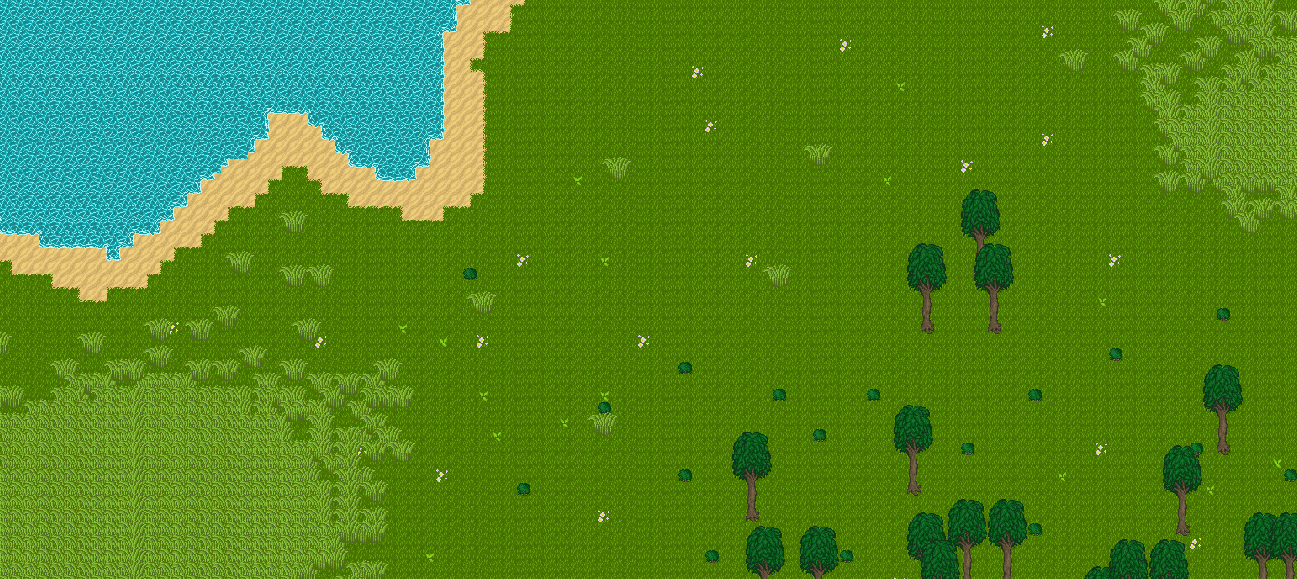
\includegraphics[width=0.8\textwidth]{assets/map.png}
      \caption{Prairie Paradise}
      \label{fig:map1}
\end{figure}

\begin{figure}[H]
      \centering
      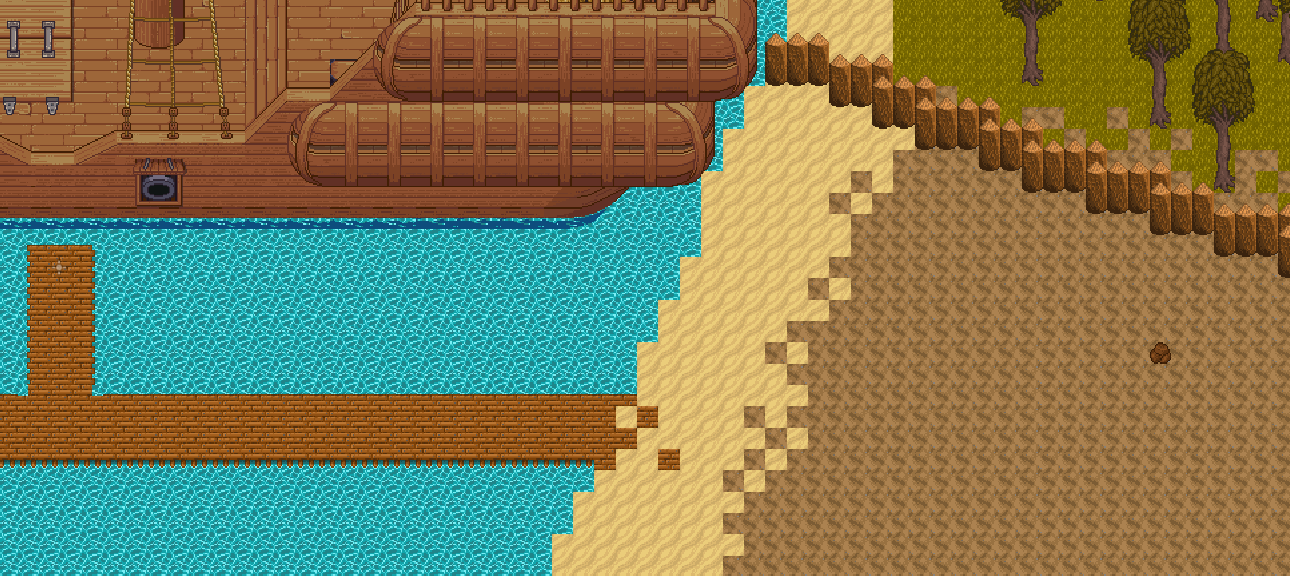
\includegraphics[width=0.8\textwidth]{assets/map2.png}
      \caption{Zone de départ}
      \label{fig:map2}
\end{figure}

\begin{figure}[H]
      \centering
      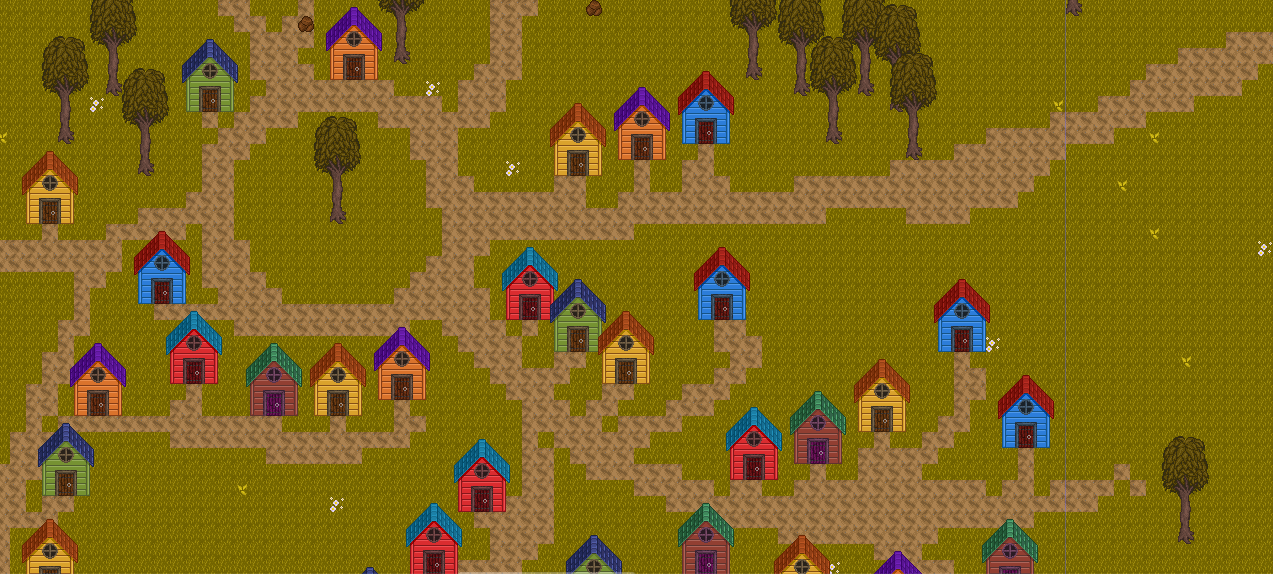
\includegraphics[width=0.8\textwidth]{assets/map3.png}
      \caption{Emberwood}
      \label{fig:map3}
\end{figure}

\subsubsection{Utilisation du logiciel GIMP}

Dans le développement de \textit{Lands of Azerith}, la création des textures a été une étape essentielle et méticuleuse, guidée par un processus rigoureux utilisant des outils avancés tels que GIMP.
Cette approche a permis d'atteindre une flexibilité créative maximale tout en assurant la cohérence visuelle et esthétique nécessaire pour immerger les joueurs dans notre monde fantastique.
\\

GIMP, un logiciel libre et puissant de manipulation d'images, a été choisi pour sa polyvalence et ses capacités avancées de création graphique.
Voici comment nous avons utilisé GIMP pour concevoir et peaufiner les textures de \textit{Lands of Azerith} :
\\

\begin{itemize}
      \item \textbf{Édition et Retouche} : GIMP nous a permis d'éditer et de retoucher chaque détail des textures avec précision.
            Des outils comme les pinceaux, les filtres et les calques ont été utilisés pour ajuster la luminosité, le contraste, et les détails des textures, garantissant ainsi une qualité visuelle optimale.
            \\

      \item \textbf{Création de Motifs et de Détails} : Nous avons utilisé les fonctionnalités avancées de GIMP pour créer des motifs complexes et des détails minutieux dans les textures.
            Cela inclut la création de motifs floraux, de structures architecturales, et d'éléments naturels comme des rochers et des arbres, intégrés de manière organique dans l'environnement du jeu.
            \\

      \item \textbf{Conversion et Exportation} : GIMP nous a également fourni des options robustes pour convertir et exporter les textures dans les formats requis par notre moteur de jeu.
            Cela inclut la gestion des formats de fichier tels que PNG, JPEG, et les formats de texture compressés comme le format DDS pour une intégration optimale dans le pipeline de développement.
\end{itemize}

\subsubsection{Processus de Création Collaboratif}

La création des textures pour \textit{Lands of Azerith} a été une initiative collaborative, impliquant des artistes graphiques, des concepteurs de niveaux et des développeurs.
Voici comment chaque étape du processus a contribué à enrichir l'expérience visuelle du jeu :
\\

\begin{itemize}
      \item \textbf{Conception Initiale} : Les artistes graphiques ont commencé par élaborer des concepts artistiques détaillés, explorant divers thèmes visuels et styles pour chaque zone de la carte. Ces concepts ont servi de base pour la création des textures finales dans GIMP.
            \\

      \item \textbf{Itérations et Révisions} : À mesure que les textures prenaient forme, des itérations et des révisions ont été effectuées en collaboration avec les concepteurs de niveaux et les développeurs pour s'assurer que les textures étaient non seulement esthétiquement plaisantes mais aussi fonctionnelles dans le contexte du jeu.
            \\

      \item \textbf{Optimisation pour les Performances} : Une attention particulière a été portée à l'optimisation des textures pour les performances du jeu. Cela inclut la gestion de la résolution des textures, la réduction de la taille des fichiers et l'utilisation efficace des techniques de compression sans compromettre la qualité visuelle.
\end{itemize}

\subsubsection{Intégration des Textures dans Godot}

Une fois les textures créées et peaufinées dans GIMP, elles ont été intégrées dans Godot, notre moteur de jeu,
pour construire les environnements interactifs de \textit{Lands of Azerith}. Voici comment cette intégration a été gérée :
\\

\begin{itemize}
      \item \textbf{Importation dans Godot} : Les textures ont été importées dans Godot en utilisant les fonctionnalités intégrées pour gérer les ressources graphiques.
            Chaque texture a été assignée aux objets correspondants dans les scènes de jeu, assurant ainsi une correspondance parfaite entre les visuels créés et les interactions du joueur.
            \\

      \item \textbf{Application des Textures} : Dans Godot, les textures ont été appliquées aux objets de manière à créer des environnements riches en détails visuels et en ambiance.
            Cela inclut la texture du sol, des murs, des objets interactifs et des éléments décoratifs qui contribuent à l'immersion globale du joueur.
\end{itemize}

\subsection{Musique et bruitages}

\subsubsection{Musiques}

Le choix de l'électro, plus précisément de la Dance électro, pour la bande sonore de \textit{Lands of Azerith} provient de son dynamisme et de sa capacité à renforcer l'énergie et l'immersion du jeu.
En sélectionnant des compositions d'artistes comme \textit{Cosmograph} et \textit{Zekk}, nous avons assuré une harmonie entre l'audio et les visuels du jeu, offrant ainsi une expérience sensorielle complète et captivante.

\subsubsection{Bande sonore}

La bande sonore de \textit{Lands of Azerith} est composée de 19 musiques existantes, sélectionnées spécifiquement pour enrichir les biomes et les situations du jeu.
\\

Chaque biome dispose de trois versions de musique : jour, nuit et combat, adaptées pour capturer l'ambiance et l'intensité des différentes phases du gameplay.
\\

Les musiques des biomes sont soigneusement conçues pour refléter l'environnement et l'atmosphère spécifiques de chaque zone du jeu. Elles contribuent à l'immersion des joueurs en créant une expérience sonore cohérente et captivante.
Les compositions musicales varient en fonction du biome, offrant une diversité d'ambiances et d'émotions pour accompagner les joueurs tout au long de leur aventure.
\\

De plus, les musiques de combat sont spécialement conçues pour intensifier l'action et l'excitation lors des affrontements avec les ennemis.
Elles sont rythmées et énergiques, créant une tension et une immersion supplémentaires pendant les combats.
\\

Enfin, les musiques de nuit apportent une atmosphère plus mystérieuse et sombre, renforçant l'exploration nocturne et offrant une expérience immersive unique.
\\

Dans l'ensemble, la bande sonore de \textit{Lands of Azerith} joue un rôle essentiel dans l'expérience globale du jeu, en créant une ambiance immersive et en renforçant l'émotion et l'immersion des joueurs dans cet univers fantastique.

\subsubsection{Exemples de Musiques de Biomes}

\begin{itemize}

      \item La musique d'ambiance de jour dans les plaines d'Emberwood capture l'atmosphère sereine et pastorale du paysage, offrant aux joueurs une immersion tranquille dans cet environnement ouvert.
            \\

      \item La version nocturne de la même musique intensifie le ton, créant une atmosphère mystérieuse et potentiellement dangereuse alors que les menaces nocturnes émergent.
            \\

      \item Pendant les combats, la musique devient plus dynamique et rythmée pour stimuler l'adrénaline des joueurs, les incitant à réagir avec précision et stratégie.
            \\

\end{itemize}

\subsubsection{Musiques des Boss et Zones Pacifiques}

Chaque boss est accompagné d'une musique distinctive et immersive, conçue pour refléter la menace et l'importance narrative de ces rencontres épiques.
Ces compositions musicales renforcent l'intensité des combats tout en enrichissant l'expérience émotionnelle des joueurs à travers des thèmes mémorables.

\subsubsection{Voix Off}

La voix off était initialement prévue pour offrir une narration riche et immersive tout au long de \textit{Lands of Azerith}.
Cependant, en raison de contraintes techniques liées au départ de la personne censée réaliser les voix, cette fonctionnalité a été modifiée.
La narration et les éléments narratifs sont maintenant intégrés dans l'environnement visuel et musical du jeu, renforçant l'immersion des joueurs à travers des visuels évocateurs et des thèmes musicaux dynamiques.

